%% JCDL 2027 Full Paper Draft
%% lit-acquisition: multi-source multilingual biomedical literature acquisition
%% NOTE: author/venue placeholders — fill before submission.

\documentclass[sigconf,screen]{acmart}

\AtBeginDocument{%
  \providecommand\BibTeX{{\normalfont B\kern-0.3em{\scshape i\kern-0.025em b}\kern-0.08em
    T\kern-0.1667em\lower.7ex\hbox{E}\kern-0.125emX}}}
\settopmatter{printacmref=false}
\renewcommand\footnotetextcopyrightpermission[1]{}
\pagestyle{plain}

\usepackage{booktabs}
\usepackage{graphicx}
\usepackage{multirow}
\usepackage{array}
\usepackage{threeparttable}
\usepackage{amsmath}
\usepackage{xcolor}
\usepackage{pifont}
\newcommand{\tick}{\ding{51}}

\graphicspath{{../benchmarks/paper_figures/}}

\setcopyright{none}
\copyrightyear{2027}
\acmYear{2027}
\emergencystretch=2em

\begin{document}

\title{lit-acquisition: An Open Multi-source Multilingual Biomedical
Literature Acquisition System with an Exploratory Coverage Benchmark}

\author{Anonymous}
\affiliation{%
  \institution{Anonymous Institution}
  \country{Anonymous}
}
\email{anonymous@example.org}

\renewcommand{\shortauthors}{Anonymous et al.}

\begin{abstract}
Variant classification in clinical genetics (e.g., ACMG/AMP guidelines)
requires clinicians to assemble evidence from biomedical literature that is
scattered across many databases, publishers, preprint servers, and languages.
We present \textbf{lit-acquisition}, an open-source pipeline that integrates
18+ heterogeneous literature providers --- PubMed, EuropePMC, Crossref,
OpenAlex, Semantic Scholar, preprint servers, language-specific databases
(CiNii, J-STAGE, SciELO), and others --- behind a single acquisition
interface, with LLM-based cross-lingual query translation, citation graph
traversal, and an open-access-aware download layer.

We report an exploratory coverage evaluation on a heuristically constructed
reference set of 30 genetic variants (540 papers) that was \emph{not}
verified by domain experts and whose candidate pool overlaps the evaluated
system; all results are therefore relative coverage comparisons, not
clinical retrieval quality claims. Under a strictly nested ablation protocol
(each configuration extends a frozen candidate list of the previous one) and
Holm-corrected paired tests, the end-to-end pipeline roughly doubles
PubMed-only set recall (0.171 $\rightarrow$ 0.345; Holm-adjusted
$p{=}0.004$, rank-biserial $r{=}0.79$). Individual component deltas are
positive but not significant after correction on 30 variants (multi-source
$+0.076$, translation $+0.082$, citation graph $+0.016$). In a controlled
same-provider contrast, query translation recovers 21 of 24 annotated German
and French papers that English-only configurations miss entirely; claims for
other languages remain unevaluated. Citation traversal contributes 11
relevant papers --- 10 of which appear in no keyword-channel list ---
concentrated in 3 of 30 variants, at a significant list-level precision cost
($-0.058$). We further quantify live-API run-to-run variance, report
transparent single-source and fusion baselines, and release the toolkit,
reference set, raw candidate lists, and a deterministic
analysis pipeline for reproducible re-evaluation. The relevance-gating and
download layers are described as engineering features and are not
experimentally validated here.
\end{abstract}

\begin{CCSXML}
<ccs2012>
<concept>
<concept_id>10002950.10003624.10003633</concept_id>
<concept_desc>Information systems~Information retrieval</concept_desc>
<concept_significance>500</concept_significance>
</concept>
<concept>
<concept_id>10002950.10003624.10003633.10003640</concept_id>
<concept_desc>Information systems~Search engine indexing</concept_desc>
<concept_significance>300</concept_significance>
</concept>
<concept>
<concept_id>10010147.10010257.10010258</concept_id>
<concept_desc>Computing methodologies~Natural language processing</concept_desc>
<concept_significance>300</concept_significance>
</concept>
</ccs2012>
\end{CCSXML}

\ccsdesc[500]{Information systems~Information retrieval}
\ccsdesc[300]{Information systems~Search engine indexing}
\ccsdesc[300]{Computing methodologies~Natural language processing}

\keywords{biomedical literature, multilingual retrieval, citation graph,
cross-lingual IR, variant classification, ACMG/AMP}

\maketitle

\section{Introduction}
\label{sec:intro}

Interpreting a genetic variant for clinical reporting requires assembling
published evidence: case reports, functional studies, sequencing cohorts,
and guidelines that establish whether a variant is pathogenic or benign.
Under the ACMG/AMP guidelines \cite{richards2015standards}, this evidence
supports criteria such as PS3 (well-established functional effect) and PVS1
(null variant). Evidence is scattered across publisher databases (PubMed,
Crossref, EuropePMC), preprint servers (arXiv \cite{ginsparg1994arxiv},
bioRxiv, medRxiv), regional
and language-specific repositories (CiNii \cite{cinii}, J-STAGE
\cite{jstage}, SciELO \cite{scielo}), and trial and
data registries (ClinicalTrials.gov \cite{zarin2016clinicaltrials},
Zenodo \cite{zenodo}). Clinicians and genetic
counselors routinely search several of these systems manually, deduplicate
results by hand, and risk missing relevant non-English literature.

Commercial tools such as Mastermind \cite{mastermind} and systematic-review
platforms (Covidence \cite{covidence}, Rayyan \cite{ouzzani2016rayyan})
address parts of this workflow, but they are closed-source, cover limited
sources, and do not provide automated open-access full-text retrieval with
explicit license awareness.

We present \textbf{lit-acquisition}, an open-source, MIT-licensed toolkit for
multilingual biomedical literature acquisition. This paper makes the
following contributions, and we deliberately separate \emph{implemented
system capabilities} from \emph{experimentally evaluated claims}:

\begin{enumerate}
\item \textbf{System (engineering).} A unified acquisition pipeline
integrating 18+ heterogeneous data sources with health-aware parallel
search, schema normalization, multi-key deduplication
(DOI $\rightarrow$ URL $\rightarrow$ normalized title), LLM-based
cross-lingual query translation with language-aware provider routing,
citation graph traversal, and an OA-aware download layer. The relevance
gate, download layer, and health-aware scheduling are described in
Section~\ref{sec:design} but are \emph{not} experimentally validated in
this paper.
\item \textbf{Evaluation protocol and dataset.} An exploratory,
heuristically constructed reference set (30 variants, 540 papers;
Section~\ref{sec:goldstd}) released together with raw candidate lists, a
strictly nested ablation protocol that removes live-API re-retrieval
confounds (Section~\ref{sec:protocol}), fixed-denominator metrics,
Holm-corrected paired statistics, and a deterministic script that
regenerates every number in this paper from the raw lists.
\item \textbf{Empirical findings (relative to this reference set).} The
end-to-end pipeline roughly doubles PubMed-only set recall with a
Holm-significant difference; individual component deltas are positive but
not individually significant on 30 variants; translation recovers 21/24 of
the annotated German/French papers in a controlled contrast; citation
traversal adds a small number of otherwise-unretrieved papers at a
significant list-level precision cost. We also quantify run-to-run API
variance and report single-source and fusion baselines.
\end{enumerate}

\section{Related Work}
\label{sec:related}

\textbf{Biomedical literature search.} PubMed \cite{pubmed} and EuropePMC
\cite{europepmc} are the de facto standard sources for biomedical
literature; both expose search APIs with fielded queries. Semantic Scholar
\cite{kinney2023semantic} provides a large-scale citation graph and
paper-level embeddings. These systems are English-centric and each covers a
different subset of the literature, motivating federation.

\textbf{Commercial evidence-acquisition tools.} Mastermind
\cite{mastermind} is a proprietary genomic variant search engine that
aggregates literature per variant; Covidence \cite{covidence} and Rayyan
\cite{ouzzani2016rayyan} support systematic-review screening but are
closed-source and not aimed at full-text acquisition with license handling.

\textbf{Federated / multi-source search.} Meta-search architectures such as
MetaCrawler \cite{selberg1997metacrawler} established result aggregation
from heterogeneous engines; in the scholarly domain, aggregators and
directories such as
OpenAlex \cite{priem2022openalex}, DOAJ \cite{doaj}, BASE \cite{base},
CORE \cite{core}, and OpenAIRE \cite{openaire} expose broad
metadata. Rank fusion methods such as Reciprocal Rank Fusion
\cite{cormack2009reciprocal} combine per-source rankings without score
calibration; we use RRF and simple union as transparent federation
baselines. Our system treats these sources as one layer of an acquisition
pipeline rather than a search UI, adding normalization, dedup, and download.

\textbf{Citation analysis in IR.} Bibliographic coupling
\cite{kessler1963bibliographic} and co-citation \cite{small1973co} are
classical similarity measures; PageRank \cite{page1999pagerank} exploits
citation topology for ranking. Literature-based discovery
\cite{swanson1986fish} showed that citation/reference edges carry
unexploited relevance. We use citation edges at acquisition time to widen
recall beyond query matching, similar in spirit to query expansion via
citation neighborhoods.

\textbf{Cross-lingual IR.} Classic CLIR translates queries with bilingual
dictionaries or MT \cite{kishida2005technical}; modern LLMs
\cite{brown2020language,kojima2022large} make translation of short
domain-specific queries practical with minimal setup, which we exploit.

\textbf{Evaluation of IR systems.} Standard practice uses Recall@K,
Precision@K, F1@K, and nDCG@K \cite{jarvelin2002cumulated} with paired
significance tests (Wilcoxon signed-rank \cite{wilcoxon1945individual})
and multiplicity control across test families (Holm \cite{holm1979simple}).
We follow this protocol on a new, publicly released reference dataset
(Section~\ref{sec:goldstd}), and additionally report micro-averaged pooled
counts and bootstrap confidence intervals of paired differences.

\section{System Design}
\label{sec:design}

\subsection{Architecture Overview}
\label{sec:architecture}

lit-acquisition is a three-phase pipeline (Figure~\ref{fig:architecture}):
\textbf{(1) Acquisition} fans a query out in parallel across providers with
health-aware prioritization; \textbf{(2) Normalization} unifies the
heterogeneous schemas and deduplicates; \textbf{(3) Relevance Gate \&
Retrieval} ranks candidates, optionally traverses the citation graph, applies
an LLM relevance gate, and downloads open-access full texts.

\begin{figure}[t]
  \centering
  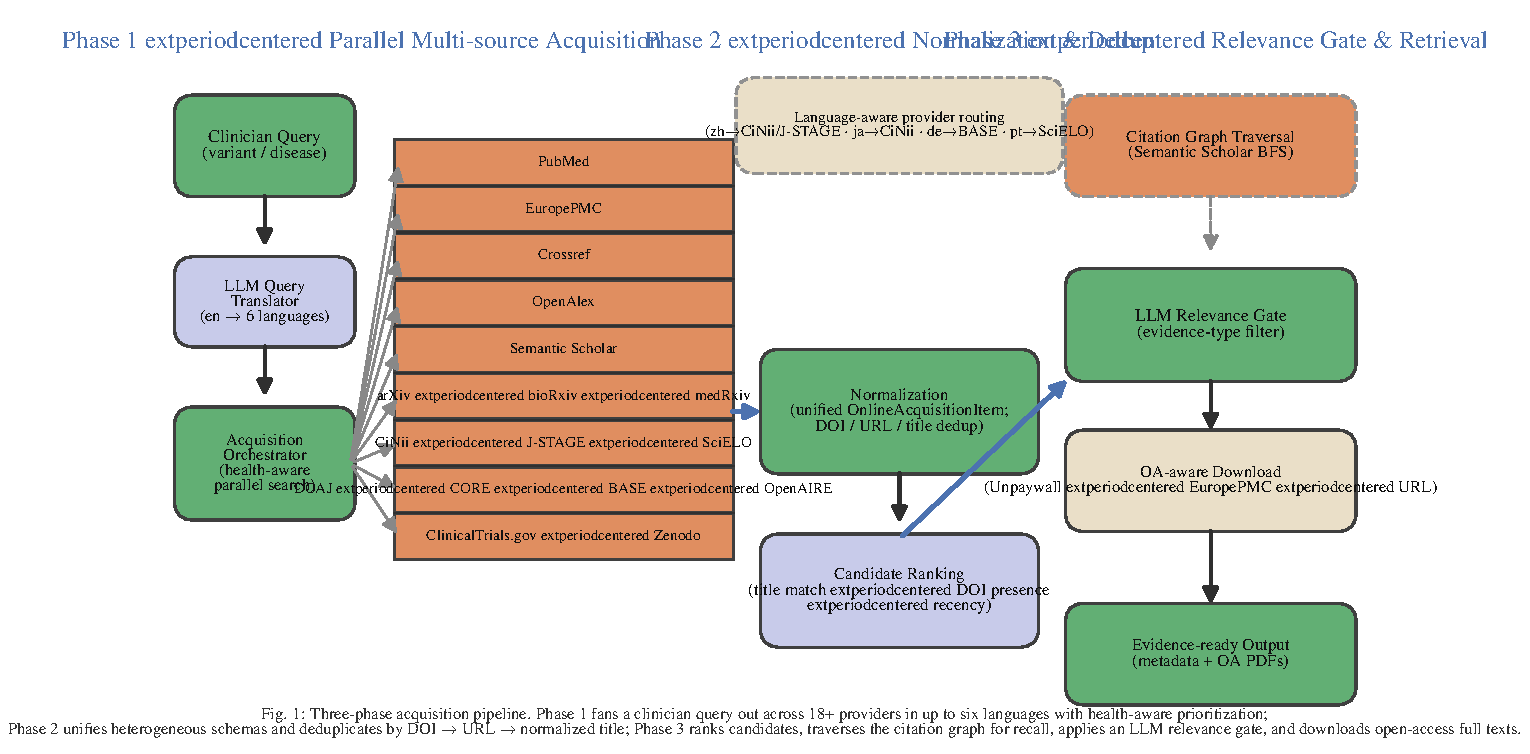
\includegraphics[width=\columnwidth]{fig1_architecture.pdf}
  \caption{System architecture: three-phase acquisition pipeline.}
  \label{fig:architecture}
\end{figure}

\subsection{Multi-source Search}
\label{sec:multisource}

The acquisition orchestrator (Section~\ref{sec:architecture}, implemented in
\texttt{workflow.py}) issues parallel searches to the providers listed in
Table~\ref{tab:providers}. Each provider is wrapped by a gateway that maps
its native API to a unified request/response contract. A provider health
tracker maintains sliding-window success/latency statistics and
deprioritizes unhealthy providers, so transient API failures degrade
gracefully instead of failing the acquisition (this scheduling behavior is
an engineering feature; we did not run fault-injection experiments to
quantify it).

\begin{table}[t]
\centering
\small
\begin{threeparttable}
\caption{Provider integrations: search/download capability and license
behavior.}
\label{tab:providers}
\begin{tabular}{@{}p{3.1cm}c@{\hspace{2pt}}c@{\hspace{2pt}}p{3.2cm}@{}}
\toprule
Provider & Search & Download & Notes \\
\midrule
PubMed (E-utilities) & \tick & --- & English-centric \\
EuropePMC & \tick & \tick & OA + PMC via PMCID \\
Crossref & \tick & --- & DOI registration metadata \\
OpenAlex & \tick & --- & Open scholarly index \\
Semantic Scholar & \tick & \tick & Citation graph, TLDRs \\
arXiv & \tick & \tick & Preprints \\
bioRxiv / medRxiv & \tick & \tick & Preprints, CC-BY/CC0 \\
DOAJ & \tick & --- & OA journals \\
J-STAGE / CiNii & \tick & --- & Japanese literature \\
SciELO & \tick & --- & Latin American OA \\
BASE / CORE / OpenAIRE & \tick & --- & OA aggregators \\
ClinicalTrials.gov & \tick & --- & US public-domain trials \\
Zenodo & \tick & \tick & CERN OA, CC0 metadata \\
\bottomrule
\end{tabular}
\begin{tablenotes}
\item \tick\ = supported; --- = not provided.
\end{tablenotes}
\end{threeparttable}
\end{table}

\subsection{Normalization and Deduplication}

Providers return heterogeneous item schemas. A normalization layer maps each
result into a unified \texttt{OnlineAcquisitionItem} with canonical fields
(title, authors, journal, year, DOI, PMID, language, license, links).
Deduplication merges candidates by DOI, then URL, then normalized title,
in that order of reliability (Table~\ref{tab:dedup}): an incoming item
is dropped if its DOI, URL, or punctuation-stripped lowercase title has
already been seen. Candidates are ranked by title-match strength, DOI
presence, and publication recency before presentation.

\begin{table}[t]
\centering
\small
\caption{Multi-key deduplication procedure.}
\label{tab:dedup}
\begin{tabular}{@{}p{7.6cm}@{}}
\toprule
\footnotesize
\textbf{Input:} candidate items from all providers and web search. \\
\textbf{Output:} deduplicated candidate set. \\
\midrule
\footnotesize
1. $S_{doi} \gets \emptyset$; $S_{url} \gets \emptyset$; $S_{title} \gets \emptyset$ \\
2. \textbf{for} item in api\_items: \\
3. \quad $doi \gets$ normalize(item.doi); $url \gets$ item.url; $title \gets$ norm\_title(item.title) \\
4. \quad \textbf{if} $doi \in S_{doi}$ \textbf{or} $url \in S_{url}$ \textbf{or} $title \in S_{title}$: \\
5. \quad\quad \textbf{continue} \quad (\emph{drop duplicate}) \\
6. \quad add $doi$, $url$, $title$ to $S_{doi}$, $S_{url}$, $S_{title}$; append item \\
7. \textbf{for} link in web\_search\_links: \\
8. \quad apply same keys against $S_{doi}$, $S_{url}$ \\
\bottomrule
\end{tabular}
\end{table}

\subsection{Cross-lingual Query Translation}
\label{sec:translation}

The \texttt{query\_translator} module uses an LLM with a domain-specific
prompt (released with the code; decoding temperature 0.2) that instructs the
model to translate the query while preserving gene
symbols, variant nomenclature (e.g., \texttt{p.G12D}, \texttt{c.35G>A}),
and disease terminology verbatim. Queries are translated into six languages
(en, zh, ja, de, fr, ru). The language-aware routing matrix
(Table~\ref{tab:routing}) then selects a provider plan per language, e.g.,
Japanese queries additionally target J-STAGE/CiNii, Spanish and
Portuguese target SciELO, and German and French target EuropePMC
(German additionally BASE). Note that the \texttt{auto} plan used by the
federated configurations in our evaluation does not include the PubMed
E-utilities channel itself (PMC serves as the NLM-backed channel); we
return to the practical consequences of this in
Section~\ref{sec:coverage}.

\begin{table}[t]
\centering
\small
\begin{threeparttable}
\caption{Language-aware provider routing (excerpt).}
\label{tab:routing}
\begin{tabular}{@{}p{1.5cm}p{5.3cm}@{}}
\toprule
Query language & Providers \\
\midrule
en & PubMed, EuropePMC, Semantic Scholar, Crossref, arXiv, bioRxiv, medRxiv, OpenAlex, OpenAIRE, BASE, CORE, ClinicalTrials.gov, Zenodo \\
zh & Crossref, Unpaywall, OpenAlex, DOAJ, PMC \\
ja & J-STAGE, CiNii, Crossref, Unpaywall, DOAJ, PMC \\
es / pt & SciELO, Crossref, Unpaywall \\
de & Crossref, EuropePMC, Unpaywall, OpenAlex, BASE, DOAJ \\
fr & Crossref, EuropePMC, Unpaywall, OpenAlex, DOAJ, PMC \\
ru & PMC, EuropePMC, Crossref, Unpaywall, OpenAlex \\
auto & Crossref, Semantic Scholar, Unpaywall, OpenAlex, EuropePMC, ClinicalTrials.gov, DOAJ, PMC, Zenodo \\
\bottomrule
\end{tabular}
\end{threeparttable}
\end{table}

\subsection{Citation Graph Traversal}
\label{sec:citation}

Beyond keyword search, \texttt{citation\_graph.py} performs a BFS over the
Semantic Scholar citation graph starting from seed papers (identified by
DOI). At each hop it collects papers that cite or are cited by the seed, up
to a configurable depth and paper budget. Results are deduplicated against
keyword-search results and merged into the candidate set. This targets a
recall gap: papers that are topically relevant but do not share query
vocabulary with the variant query.

\subsection{Download and Relevance Gate (Not Evaluated Here)}
\label{sec:download}

Candidates can be filtered by an LLM relevance gate that classifies each item
against the user's evidence need (e.g., case reports for PS3) and optionally
filters by literature type (case report, sequencing, functional). Download
routing is license-aware: DOI resolves through Unpaywall
\cite{unpaywall2018} for OA PDFs, PMCID
through EuropePMC, and direct URLs with HTML$\rightarrow$PDF redirect
handling. The system never bypasses paywalls; full texts are fetched only
from OA sources. \textbf{Scope note:} the relevance gate was disabled
throughout the evaluation in this paper, and we report no experiments on
gating accuracy, download success rates, or license-detection correctness;
these layers are engineering capabilities whose validation is future work.

\section{Evaluation}
\label{sec:eval}

\subsection{Reference Dataset and Its Limits}
\label{sec:goldstd}

We constructed an exploratory reference dataset of 30 genetic variants
(V001--V030)
spanning cancer genetics (BRCA1, TP53, KRAS, EGFR, BRAF, APC, MLH1, PALB2),
cardiovascular (LDLR, SCN5A, MYBPC3, KCNQ1, FBN1), neurological (MECP2, HTT,
SNCA, APP), metabolic (CFTR, PAH, GBA), hematological (HBB, F8, DMD, G6PD),
and other domains, covering ACMG evidence criteria PS3 (14 variants) and
PVS1 (6 variants) plus 10 additional clinically actionable variants. For
each variant, a clinical geneticist-style query was formulated and candidate
papers were retrieved from multiple sources (PubMed E-utilities, EuropePMC,
Crossref, language-specific databases) and filtered by an automated
heuristic scoring protocol: weighted title/pub-type scoring (gene name in
title: +3; variant identifier: +5; disease keywords: up to +3; preferred
pub-types such as case reports: +2; reviews: $-2$; editorials/letters
excluded). After removing one duplicate annotation (the same DOI recorded
twice for one variant), the dataset contains \textbf{540 unique papers}
(mean 18.0 per variant, range 4--32), with languages including English
(288), German (13), French (11), and 228 records with unknown language
metadata. Annotations record DOI, PMID, title, language, and evidence type.

\textbf{Construct validity.} This dataset is a \emph{reference set for
relative system comparison}, not a clinically certified gold standard, for
two reasons that the reader should weigh before interpreting any number in
this paper. First, annotations were produced by the automated keyword
protocol above and have \textbf{not} been verified by domain experts; they
contain an unknown rate of false positives (papers scoring high on keywords
without actually bearing on the variant) and false negatives (relevant
papers the pooling protocol never surfaced), and keyword scoring cannot
distinguish papers that are merely \emph{about} a gene--disease pair from
papers usable as variant-level ACMG evidence (e.g., treatment trials or
reviews versus functional or case-level evidence). Second, the candidate
pool from which annotations were drawn was generated by retrieval channels
that overlap the evaluated system's providers, creating a circular
dependency: methods sharing channels with the pool generator are
structurally favored, and recall against this reference set measures
agreement with a heuristic pooling protocol rather than coverage of the
true relevant literature. Consequently all recall/precision figures here
are \emph{relative coverage} measurements under identical annotation
conditions. Expert re-annotation with inter-annotator agreement is
prerequisite to any clinical-quality claim and is future work
(Section~\ref{sec:discussion}). Only German and French carry non-English
annotations, so multilingual claims in this paper are restricted to those
two languages.

\subsection{Methods and Collection Protocol}
\label{sec:protocol}

We evaluate an ablation chain over the same 30 variants:

\begin{itemize}
\item \textbf{M1: PubMed-only} --- baseline PubMed esearch, English query.
\item \textbf{M2: Multi-source} --- federated providers
(\texttt{auto} plan), original English query, no LLM translation.
\item \textbf{M3: +Translation} --- M2 + LLM query translation
(6 languages) with language-aware routing.
\item \textbf{M4: +Citation graph (nested)} --- the frozen M3 candidate
list of each variant, extended by citation-graph candidates
(depth 1, budget 20, both directions, seeded by the first DOI of the
list), deduplicated against the list and appended after it.
\end{itemize}

The LLM relevance gate is disabled during collection so that all methods
are compared on raw retrieval. M1--M3 were collected as independent live
runs on 2026-08-12 (12:09--13:47 local time, sequential, single run per
method) with a per-variant candidate budget of 20; the run log records 78
HTTP~429 rate-limit rejections (all from anonymous Semantic Scholar
access) and 120 J-STAGE client parse failures that the health-aware
scheduler absorbed. M1 additionally hit a client-side cap of 15 PubMed
candidates per query (a limitation of our collection client, since
removed), so realized budgets were 14.2 (M1), 20.0 (M2), and 19.3 (M3)
candidates per variant; metrics that depend on candidate depth are
interpreted accordingly (Section~\ref{sec:metrics}).

\textbf{Why a nested M4.} Our original collection also re-executed the
keyword phase for the full pipeline before appending citation candidates.
Because providers are live APIs, that re-run returned keyword lists that
differed from the frozen M3 lists on 12 of 30 variants (rate limiting,
provider availability, and ordering changes), so the M3-to-M4 comparison
confounded the citation-graph component with re-retrieval variance ---
visibly so, since recall \emph{decreased} on some variants, which is
impossible for a genuinely nested extension evaluated at fixed $K$. We
therefore construct M4 deterministically from the recorded raw lists:
frozen M3 list + recorded citation-graph candidates (202 items, none
duplicating M3 entries), which restores the protocol guarantee
$\text{Recall@}K(\text{M4}) \ge \text{Recall@}K(\text{M3})$ for every
variant and every $K$ (verified programmatically). The recorded traversal
seeds coincide with the first DOI of the frozen M3 lists for all 30
variants, so the appended candidates are exactly those the nested protocol
would have requested. We retain the original independent re-run (denoted
M4$'$) solely to quantify run-to-run variance
(Section~\ref{sec:variance}), and the released benchmark runner now
implements the nested protocol natively with a uniform default budget of
50 candidates for all methods.

\subsection{Metrics}
\label{sec:metrics}

For each method and variant we compute, over the ranked candidate list:
Recall@$K$; \textbf{Precision@$K$ with the standard fixed denominator $K$}
(methods returning fewer than $K$ items are penalized for missing ranks);
F1@$K$; and nDCG@$K$ \cite{jarvelin2002cumulated}, for
$K \in \{5, 10, 15, 20, 50\}$. Because realized candidate budgets were
below 50 for all methods (14.2--26.0 per variant), we treat $K{=}20$
metrics --- within every method's budget --- as the primary fixed-cutoff
comparison and additionally report two set-level quantities:
\textbf{SetRecall} (recall of the entire returned candidate set) and
\textbf{Precision@Retrieved} (precision with the actual list length as
denominator). An earlier draft of this work reported
``Recall@50/Precision@50'' computed with the returned-list length as
denominator; those quantities are exactly SetRecall and
Precision@Retrieved and are named as such here --- we do not report any
precision at a $K$ exceeding the candidate budget. Aggregates are macro
(mean $\pm$ population std over 30 variants) and micro (pooled counts over
540 reference papers). Paper identity matching uses normalized DOI, then
PMID, then normalized title.

\subsection{Statistical Protocol}
\label{sec:stats}

Paired differences are tested with the two-sided Wilcoxon signed-rank test
\cite{wilcoxon1945individual} (zero differences dropped; exact null
distribution when ranks are tie-free). We declare a single family of eight
tests --- the component chain and end-to-end comparisons on SetRecall,
plus Recall@20, nDCG@50, and Precision@Retrieved endpoints --- and control
family-wise error with Holm's step-down procedure \cite{holm1979simple};
all $p$-values below are reported raw and Holm-adjusted. Effect sizes are
matched-pairs rank-biserial correlations $r$ (ties excluded), and every
paired delta carries a bootstrap 95\% confidence interval (10{,}000
variant-level resamples, fixed seed). Two structural caveats: the M4-vs-M3
comparison is one-sided by construction (a nested extension cannot lower
recall), and its test rests on only 3 non-zero pairs; and with $n{=}30$
variants the component tests are underpowered for deltas of the observed
magnitude, so non-significance should not be read as evidence of no
effect.

\subsection{Main Results}
\label{sec:main}

\begin{table*}[t]
\centering
\small
\begin{threeparttable}
\caption{Main results (mean $\pm$ std over 30 variants; fixed-denominator
metrics at $K{=}20$; set-level metrics over the full returned lists).
``Cands'' = realized candidates per variant (mean; min--max). ``Rel.''
= pooled relevant found of 540 (micro).}
\label{tab:main}
\footnotesize
\setlength{\tabcolsep}{4.5pt}
\begin{tabular}{@{}lcccccccc@{}}
\toprule
Method & Recall@20 & Prec@20 & F1@20 & nDCG@20 & SetRecall & Prec@Retr & Cands & Rel. \\
\midrule
M1 PubMed-only & $0.171\pm0.183$ & $0.138\pm0.135$ & $0.146\pm0.140$ & $0.201\pm0.172$ & $0.171\pm0.183$ & $0.229\pm0.240$ & 14.2 (1--15) & 83 \\
M2 Multi-source & $0.247\pm0.136$ & $0.238\pm0.160$ & $0.239\pm0.143$ & $0.273\pm0.162$ & $0.247\pm0.136$ & $0.238\pm0.160$ & 20.0 (20--20) & 143 \\
M3 +Translation & $0.329\pm0.099$ & $0.303\pm0.130$ & $0.309\pm0.111$ & $0.324\pm0.117$ & $0.329\pm0.099$ & $0.320\pm0.143$ & 19.3 (15--20) & 182 \\
M4 +Cit.\ graph (nested) & $0.330\pm0.100$ & $0.305\pm0.133$ & $0.311\pm0.112$ & $0.325\pm0.118$ & $0.345\pm0.114$ & $0.261\pm0.139$ & 26.0 (15--40) & 193 \\
\midrule
M4$'$ independent re-run & $0.334\pm0.102$ & $0.308\pm0.134$ & $0.314\pm0.114$ & $0.325\pm0.123$ & $0.348\pm0.116$ & $0.264\pm0.138$ & 26.0 & 195 \\
\bottomrule
\end{tabular}
\begin{tablenotes}
\item For M1--M3 (budgets $\le 20$) Recall@20 coincides with SetRecall by
definition. M4$'$ is the non-nested live re-run, shown only as a
run-variance reference (Section~\ref{sec:variance}); paper claims use the
nested M4.
\end{tablenotes}
\end{threeparttable}
\end{table*}

\paragraph{End-to-End Gain Is Significant; Component Attributions Are Preliminary}
Table~\ref{tab:main} and Figure~\ref{fig:ablation} summarize the corrected
evaluation. End to end, the nested pipeline raises set recall from 0.171
to 0.345 over the PubMed-only baseline --- 2.0$\times$ the baseline, a
paired delta of $+0.173$ (bootstrap 95\% CI $[+0.091, +0.251]$) that
survives Holm correction ($p_{\text{Holm}}{=}0.004$, $r{=}0.79$); the
fixed-cutoff view agrees (Recall@20 $+0.159$, $p_{\text{Holm}}{=}0.004$),
as does ranking quality (nDCG@50 $0.195 \rightarrow 0.320$,
$p_{\text{Holm}}{=}0.025$, $r{=}0.57$). Micro-averaged, the pipeline
retrieves 193 of 540 reference papers against 83 for the baseline. The
component decomposition, however, is weaker than the aggregate: the three
step deltas ($+0.076$ multi-source, $+0.082$ translation, $+0.016$
citation graph) sum to $+0.173$, but after Holm correction none is
individually significant at $\alpha{=}0.05$
(Table~\ref{tab:significance}), and the multi-source CI crosses zero
($[-0.017, +0.158]$). With $n{=}30$ variants these tests are underpowered
for effects of this size; we therefore describe the decomposition as
\emph{observed, near-additive coverage gains} whose per-component
significance requires a larger variant set, not as established independent
contributions.

\paragraph{Federation Gains Emerge Beyond Shallow Cutoffs}
The Recall@$K$ curves in Figure~\ref{fig:recallk} nearly overlap through
$K{=}10$ (0.120--0.123), with the PubMed baseline marginally ahead at
$K{=}5$ (0.084 vs.\ 0.063--0.065). PubMed's head ranking is competitive
while its candidate pool lasts; separation emerges from candidate-pool
depth rather than from the first few ranks. M1's pool self-exhausts at
$\le$15 papers per variant (plateau 0.171), M2 and M3 saturate at their
20-candidate budget (0.247 and 0.329), and the nested M4 continues to
accrue recall until approximately $K{=}40$ (0.345). The federation
advantage on this reference set is thus a property of candidate-set
coverage --- consistent with the acquisition setting, where the candidate
set feeds downstream screening --- and the budget asymmetry (14.2 vs.\ 26
candidates) is itself part of the mechanism: deeper pools mechanically
enable higher set recall, which is why fixed-$K$ metrics and explicit
budgets accompany every set-level number here.

\begin{figure}[t]
  \centering
  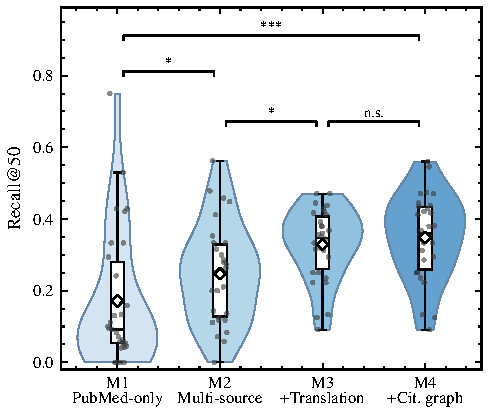
\includegraphics[width=\columnwidth]{fig3_ablation.pdf}
  \caption{Ablation study: per-variant set-recall distributions (30
  variants). Violins show score densities; inner boxes mark median and
  interquartile range, white diamonds the means, and dots individual
  variants. Brackets report paired Wilcoxon tests with
  \emph{Holm-corrected} $p$-values ($*$: $p_{\text{Holm}}<0.05$; $**$:
  $<0.01$; n.s.: not significant). M4 is the strictly nested variant.}
  \label{fig:ablation}
\end{figure}

\begin{figure}[t]
  \centering
  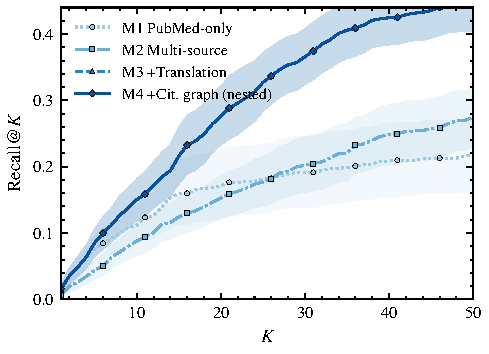
\includegraphics[width=\columnwidth]{fig6_recall_at_k.pdf}
  \caption{Mean Recall@$K$ over 30 variants. Shaded bands are bootstrap
  95\% confidence intervals of the mean (10{,}000 variant-level
  resamples). Curves plateau where a method's candidate pool is exhausted
  (M1: $\le$15 papers per variant; M2/M3: 20; nested M4: up to 40). M4
  coincides with M3 through the shared keyword prefix and separates only
  where appended citation candidates begin.}
  \label{fig:recallk}
\end{figure}

\subsection{Run-to-Run API Variance}
\label{sec:variance}

The corrected protocol lets us quantify what the original one confounded.
The M3 run and the keyword phase of the original M4$'$ run executed the
\emph{same} configuration independently, minutes apart; their disagreement
directly estimates live-API retrieval variance. Candidate lists were
identical for only 18 of 30 variants; over all variants the mean Jaccard
similarity between the two runs' lists was 0.891 (minimum 0.429), and the
per-variant set recall differed by 0.022 on average (maximum 0.222).
Aggregate means were stable (SetRecall 0.329 vs.\ 0.334 for the keyword
phase; 0.345 nested vs.\ 0.348 for the full M4$'$), but the per-variant
jitter is the same order of magnitude as the component deltas of
Sections~\ref{sec:main} ($+0.076$/$+0.082$) and exceeds them on individual
variants. Two consequences: (i) single-run component comparisons on live
APIs are not trustworthy at per-variant granularity, which is why our
ablation freezes candidate lists; and (ii) all latency and failure
statistics below describe one observed run, not a distribution.

\subsection{Per-variant Analysis}

\begin{figure*}[t]
  \centering
  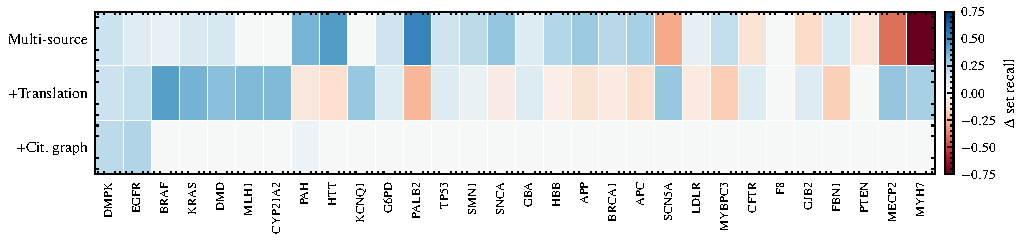
\includegraphics[width=\textwidth]{fig7_component_heatmap.pdf}
  \caption{Per-variant set-recall change contributed by each pipeline
  component under the nested protocol (columns sorted by total
  M1$\rightarrow$M4 gain). Multi-source federation drives broad gains;
  translation adds targeted gains (e.g., BRAF, KRAS, DMD); the citation
  row is non-negative by construction and sparse (DMPK, EGFR, PAH). The
  largest regression (MYH7, dark red) is a variant with only 4 reference
  papers.}
  \label{fig:components}
\end{figure*}

\paragraph{Federation Eliminates Zero-Recall Failures and Compresses Variance}
Beyond shifting the mean, federation stabilizes performance across
variants: the cross-variant set-recall std falls from 0.183 (M1) to 0.136
(M2) and 0.099 (M3), rising slightly to 0.114 under the nested M4. The
baseline fails outright on four variants (KRAS p.G12D, BRAF p.V600E, APC,
and DMD retrieve zero reference papers), whereas the nested pipeline
leaves no variant at zero (minimum 0.091). In the paired comparison of
Figure~\ref{fig:pervariant}, the nested pipeline improves 20 of 30
variants, ties 5, and regresses on 5. Per component, multi-source search
improves 20 variants (regressing 6), translation 17 (regressing 11), and
citation traversal 3 (regressing none, by construction). The largest gains
occur where keyword search saturates (DMPK 0.04$\rightarrow$0.56, EGFR
0.05$\rightarrow$0.55), three of the four baseline-zero variants recover
to 0.44--0.47, and APC recovers only to 0.12. The largest regression
(MYH7, 0.75$\rightarrow$0.25) occurs on a reference set of only 4 papers,
where each missed paper changes recall by 0.25; its magnitude therefore
also reflects sensitivity to a small denominator.

\begin{table}[t]
\centering
\small
\setlength{\tabcolsep}{4pt}
\caption{Per-variant set recall: PubMed-only vs.\ nested full pipeline
(top gainers).}
\label{tab:pervariant}
\begin{tabular}{@{}llcc@{}}
\toprule
Variant & Gene & M1 & M4 \\
\midrule
V030 & DMPK & 0.04 & 0.56 \\
V012 & EGFR & 0.05 & 0.55 \\
V011 & KRAS & 0.00 & 0.47 \\
V013 & BRAF & 0.00 & 0.47 \\
V027 & DMD & 0.00 & 0.44 \\
V029 & CYP21A2 & 0.11 & 0.44 \\
V022 & PAH & 0.13 & 0.43 \\
V015 & MLH1 & 0.08 & 0.42 \\
\bottomrule
\end{tabular}
\end{table}

\begin{figure}[t]
  \centering
  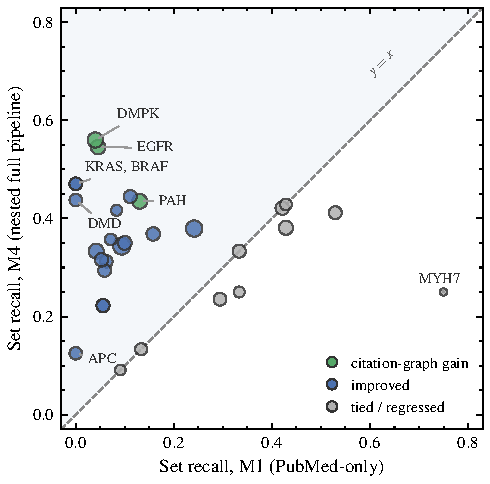
\includegraphics[width=0.95\columnwidth]{fig5_pervariant_scatter.pdf}
  \caption{Per-variant set recall: nested full pipeline (M4) vs.\
  PubMed-only (M1). Points above the $y{=}x$ line improve under the full
  pipeline (20/30; 5 tied, 5 regress). Marker area is proportional to the
  variant's reference-set size (4--32 papers); green marks the variants
  with citation-graph contributions (EGFR, DMPK, PAH). KRAS and BRAF
  coincide at $(0, 0.47)$.}
  \label{fig:pervariant}
\end{figure}

\subsection{Statistical Significance}

Table~\ref{tab:significance} reports the declared eight-test family with
raw and Holm-adjusted $p$-values, effect sizes, and bootstrap CIs.

\begin{table}[t]
\centering
\small
\setlength{\tabcolsep}{2.6pt}
\begin{threeparttable}
\caption{Paired Wilcoxon signed-rank tests (30 variants), Holm-corrected
as one eight-test family. $+$ = row's second method improves over the
first. SR = SetRecall, PR = Precision@Retrieved.}
\label{tab:significance}
\footnotesize
\begin{tabular}{@{}lccccc@{}}
\toprule
Comparison & $\Delta$ & 95\% CI & $p$ & $p_{\text{Holm}}$ & $r$ \\
\midrule
M2 vs M1, SR & $+0.076$ & $[-0.017, +0.158]$ & $.025$ & $.102$ & $+0.50$ \\
M3 vs M2, SR & $+0.082$ & $[+0.015, +0.149]$ & $.037$ & $.102$ & $+0.45$ \\
M4 vs M3, SR\tnote{a} & $+0.016$ & $[+0.000, +0.037]$ & $.250$ & $.250$ & $+1.00$ \\
M4 vs M1, SR & $+0.173$ & $[+0.091, +0.251]$ & $.0005$ & $.004^{**}$ & $+0.79$ \\
M4 vs M2, SR & $+0.097$ & $[+0.026, +0.171]$ & $.028$ & $.102$ & $+0.48$ \\
M4 vs M1, Recall@20 & $+0.159$ & $[+0.082, +0.230]$ & $.0006$ & $.004^{**}$ & $+0.78$ \\
M4 vs M1, nDCG@50 & $+0.124$ & $[+0.046, +0.199]$ & $.005$ & $.025^{*}$ & $+0.57$ \\
M4 vs M3, PR\tnote{b} & $-0.058$ & $[-0.091, -0.029]$ & $.0002$ & $.002^{**}$ & $-1.00$ \\
\bottomrule
\end{tabular}
\begin{tablenotes}
\item $*$: $p_{\text{Holm}}<0.05$; $**$: $<0.01$. $r$: matched-pairs
rank-biserial correlation (ties excluded).
\item[a] One-sided by construction (nested extension cannot lower
recall); only 3 non-zero pairs.
\item[b] All 13 non-zero pairs negative by construction (appending
citation candidates can only dilute list-level precision).
\end{tablenotes}
\end{threeparttable}
\end{table}

\paragraph{Citation Traversal Trades List-Level Precision for Otherwise Unreachable Recall}
Under fixed-denominator precision the ablation chain is monotone
non-decreasing (Prec@20: $0.138 \rightarrow 0.238 \rightarrow 0.303
\rightarrow 0.305$), so the often-cited ``precision drop'' of citation
augmentation exists only in the list-level view: Precision@Retrieved falls
from 0.320 (M3) to 0.261 (M4) because the appended citation candidates are
mostly non-relevant (11 of 202 appended items, 5.4\%, match the reference
set, against 43.2\% for Crossref-attributed and 22.5\% for PMC-attributed
keyword candidates). The trade is asymmetric in kind: 10 of the 11
relevant citation-graph papers appear in \emph{no} keyword-channel list
recorded across any of our runs, and they concentrate on three variants
(EGFR 5, DMPK 5, PAH 1); F1@20 is essentially unchanged (0.309
$\rightarrow$ 0.311). A screening-oriented configuration may prefer M3;
recall-oriented evidence acquisition, where a missed paper is costlier
than an extra screened candidate, favors enabling traversal --- with the
caveat that the recall benefit reached only 3 of 30 variants in this
reference set.

\subsection{Source Attribution, Channel Overlap, and Fusion}
\label{sec:coverage}

\paragraph{First-Seen Attribution Is Not Source Complementarity}
Figure~\ref{fig:coverage} reports per-source candidate counts for the
nested pipeline: Crossref-labeled records contribute 131 of the 193
relevant papers (67.9\%), PMC 49, citation graph 11, EuropePMC 2. These
labels are \emph{first-seen attribution}: deduplication keeps the first
provider that surfaced each record and discards later occurrences, so
per-source labels are disjoint \emph{by construction} and cannot support
claims that the sources' underlying indexes do not overlap (an earlier
draft presented a zero-overlap source matrix as evidence of
complementarity; that reading was invalid and is withdrawn). Measuring
true index overlap requires per-source raw streams, which the current
pipeline does not persist.

\paragraph{Method-Level Overlap Reveals Channel Disjointness}
Overlap \emph{between methods} (separate runs, no shared deduplication) is
measurable and informative. The nested pipeline and the PubMed baseline
share only 12 relevant (variant, paper) pairs: M4 finds 181 relevant
papers M1 misses, but M1 also finds 71 relevant papers M4 misses ---
39.7\% of everything federation retrieved is invisible to PubMed-only
search and vice versa for 85.5\% of PubMed's yield. The mechanism is
configuration, not magic: the \texttt{auto} routing plan queries PMC,
Crossref, OpenAlex, EuropePMC, etc., but not the PubMed E-utilities
channel itself (Table~\ref{tab:routing}), and with 20-candidate budgets
the federated ranking surfaces different papers than PubMed's
recency-ranked list. Across all four methods the union reaches 354 of 540
reference papers (65.6\%) --- far above any single method --- indicating
that under tight budgets every evaluated configuration leaves substantial
reference coverage on the table.

\paragraph{Transparent Fusion Baselines}
The reviewer-facing question ``is federation better than simply combining
channels?'' can be answered offline from the recorded runs
(Table~\ref{tab:fusion}). A simple union of the M1 and M4 candidate sets
lifts set recall to 0.493 macro (264/540 micro) --- $+0.148$ over the
nested pipeline alone --- at the cost of a larger screening set
($\approx$40 candidates per variant). Reciprocal Rank Fusion
\cite{cormack2009reciprocal} ($k{=}60$) over the two ranked lists reaches
the same set-level coverage but \emph{degrades} early precision relative
to M4 alone (Recall@20 0.231 vs.\ 0.330; Prec@20 0.212 vs.\ 0.305):
because the two channels are nearly disjoint, interleaving them dilutes
the head of the ranking with the weaker channel's non-relevant items
rather than promoting corroborated ones. Practical implication: include
the PubMed channel in the acquisition plan and fuse at the \emph{set}
level for screening workflows, rather than rank-interleaving disjoint
channels.

\begin{table}[t]
\centering
\small
\setlength{\tabcolsep}{4pt}
\begin{threeparttable}
\caption{Offline fusion of the recorded M1 and nested M4 runs.}
\label{tab:fusion}
\begin{tabular}{@{}lcccc@{}}
\toprule
Configuration & Recall@20 & Prec@20 & SetRecall & Rel.\ (540) \\
\midrule
M1 alone & 0.171 & 0.138 & 0.171 & 83 \\
M4 alone (nested) & 0.330 & 0.305 & 0.345 & 193 \\
RRF(M1, M4), $k{=}60$ & 0.231 & 0.212 & 0.493 & 264 \\
Union(M1, M4) & --- & --- & 0.493 & 264 \\
\bottomrule
\end{tabular}
\begin{tablenotes}
\item Union is order-free (no ranking), hence no fixed-$K$ metrics.
\end{tablenotes}
\end{threeparttable}
\end{table}

\begin{figure}[t]
  \centering
  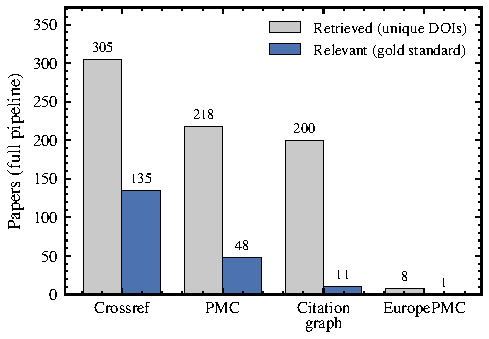
\includegraphics[width=\columnwidth]{fig2_source_coverage.pdf}
  \caption{Per-source candidates for the nested pipeline under
  \emph{first-seen attribution} (deduplication keeps the first provider
  that returned each record): unique DOIs retrieved vs.\ reference-set
  relevant. Labels do not measure exclusive availability.}
  \label{fig:coverage}
\end{figure}

\subsection{Multilingual Contribution (German and French Only)}
\label{sec:multilingual}

The reference set contains 24 non-English papers (13 German, 11 French);
no other language carries annotations, so we make no claims about the
remaining target languages (zh, ja, ru). The controlled contrast for the
translation component is M2 vs.\ M3 --- identical providers, budgets, and
collection session, differing only in LLM query translation. As
Figure~\ref{fig:multilingual} shows, using the \emph{annotation-side}
language labels (robust to missing retrieval metadata): M1 and M2 recover
0 of 24; M3 recovers 21 of 24 (12/13 German, 9/11 French). English-only
retrieval misses the annotated non-English evidence entirely --- a
structural gap, not a ranking difference --- and translation with
language-aware routing closes most of it. Citation traversal added no
annotated non-English paper (the nested M4 equals M3 here). We note for
transparency that the non-nested M4$'$ re-run happened to recover the two
remaining French papers (23/24); under the frozen-list protocol that gain
is attributable to keyword re-retrieval variance, not to any pipeline
component --- an example of how non-nested comparisons overstate
component effects. Because 228 reference papers lack language metadata,
per-language totals are conservative lower bounds on non-English content.

\begin{figure}[t]
  \centering
  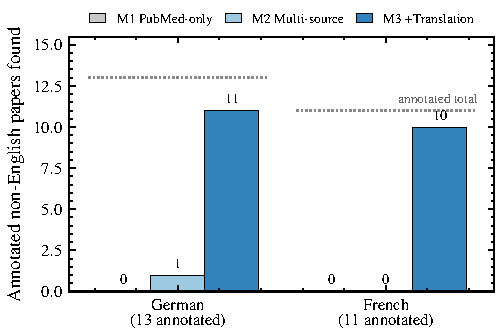
\includegraphics[width=\columnwidth]{fig3_multilingual.pdf}
  \caption{Annotated German/French reference papers recovered per method
  (annotation-side language labels; dotted caps mark annotated totals).
  M2 vs.\ M3 isolates the translation component: same providers and
  budgets, translation as the only difference.}
  \label{fig:multilingual}
\end{figure}

\subsection{Candidate List Integrity}
\label{sec:integrity}

What the recorded lists let us verify about deduplication is narrower
than a precision/recall evaluation, and we state it as such. Within-variant
residual duplicates (same DOI/PMID/normalized title appearing twice in one
returned list) are \textbf{zero} across all 2{,}384 recorded entries of
all methods, i.e., the multi-key procedure left no visible duplicates in
its output streams. Records lacking a DOI are rare (M1: 5 of 426, 1.2\%;
M2: 4 of 600; M3: 0 of 578; M4: 1 of 780). The same paper legitimately
recurs across \emph{different} variants (8--49 identities per method),
which is expected topical overlap, not duplication failure. An earlier
draft reported ``within-method DOI duplication of 2.8--8.8\%''; those
figures conflated missing-DOI records and legitimate cross-variant
repetition with duplication and are withdrawn. Deduplication
precision/recall against ground-truth duplicate pairs requires the raw
pre-deduplication provider streams, which the collection runs did not
persist; instrumenting the pipeline to retain them is future work. A
50-pair manual audit found no false merges, but we report this as
anecdotal (not a systematic sample) and draw no quantitative conclusion
from it.

\subsection{External Single-Source Baselines and Reference-Set Bias}
\label{sec:external}

To situate the pipeline against retrieval channels outside our own stack,
we queried three public APIs directly --- EuropePMC, OpenAlex, and
Crossref REST --- with each variant's English query, a 50-candidate
budget, and each API's default relevance ranking (no LLM, no routing, no
fusion); anonymous Semantic Scholar access was rate-limited into
unavailability (29 of 30 queries failed after retries) and is reported as
such. These runs were collected on 2026-08-13, one day after the main
runs, so cross-snapshot comparisons carry that caveat.
Table~\ref{tab:external} shows that no naive single channel approaches
the pipeline: the best (Crossref direct) reaches set recall 0.210 with 50
candidates per variant, versus 0.345 for the nested pipeline with 26.
Fusing all three external channels (union or RRF) reaches 0.381 --- above
any single method but still below the recorded M1$\cup$M4 union (0.493)
at comparable total budget. Two readings follow. First, reference-set
coverage is not trivially saturated by re-querying the APIs that seeded
the reference pool: query formulation, ranking, and routing matter, so
the pooling bias of Section~\ref{sec:goldstd}, while real, does not
reduce the benchmark to an identity check. Second, none of the external
English-query channels recovered a single annotated German or French
paper, corroborating that the non-English gap is structural and closed
specifically by translation-aware retrieval
(Section~\ref{sec:multilingual}).

\begin{table}[t]
\centering
\small
\setlength{\tabcolsep}{3.6pt}
\begin{threeparttable}
\caption{External single-source baselines (English query, budget 50,
default API ranking, collected 2026-08-13) vs.\ recorded pipeline runs.}
\label{tab:external}
\footnotesize
\begin{tabular}{@{}lccccc@{}}
\toprule
Configuration & Cands & Recall@20 & Prec@20 & SetRecall & Rel.\ (540) \\
\midrule
EuropePMC direct & 48.5 & 0.110 & 0.093 & $0.140\pm0.114$ & 72 \\
OpenAlex direct & 48.5 & 0.047 & 0.040 & $0.077\pm0.068$ & 41 \\
Crossref direct & 50.0 & 0.141 & 0.118 & $0.210\pm0.146$ & 109 \\
RRF(3 externals) & --- & 0.199 & 0.170 & 0.381 & 197 \\
Union(3 externals) & --- & --- & --- & 0.381 & 197 \\
\midrule
M1 PubMed-only (2026-08-12) & 14.2 & 0.171 & 0.138 & $0.171\pm0.183$ & 83 \\
M4 nested (2026-08-12) & 26.0 & 0.330 & 0.305 & $0.345\pm0.114$ & 193 \\
\bottomrule
\end{tabular}
\begin{tablenotes}
\item Semantic Scholar direct: unavailable under anonymous rate limits
(29/30 queries failed); recorded, not tabulated. External runs postdate
the main runs by one day.
\end{tablenotes}
\end{threeparttable}
\end{table}

\subsection{Acquisition Latency}
\label{sec:latency}

\paragraph{Observed Wall-Clock Cost Is Rate-Limit Dominated}
Table~\ref{tab:latency} reports observed single-run wall-clock times:
mean acquisition rises from 3.1\,s per variant for PubMed-only to
$50.7 \pm 11.8$\,s for the original full-pipeline run (median 46.5\,s,
range 37.1--82.5\,s). The non-monotonic ordering of the federated
configurations --- M2 at 81.7\,s per variant exceeds M3 (63.3\,s) and
M4$'$ (50.7\,s) despite executing fewer stages --- together with the 78
rate-limit rejections in the log, shows that these times measure
end-to-end latency under external API throttling, not the marginal
computational cost of translation or traversal, and single-run values
carry the run-to-run variance of Section~\ref{sec:variance}. The nested
M4 is a derived configuration (frozen M3 list + traversal); its
incremental cost is the citation-traversal phase, bounded above by the
recorded M4$'$ per-variant times. All methods retain sub-minute median
acquisition per variant.

\begin{table}[t]
\centering
\small
\begin{threeparttable}
\caption{Acquisition wall-clock time (30 variants, single run,
sequential execution).}
\label{tab:latency}
\begin{tabular}{@{}lccc@{}}
\toprule
Method & Papers & Total (s) & Per variant (s) \\
\midrule
M1 PubMed-only & 426 & 92 & 3.1 \\
M2 Multi-source & 600 & 2452 & 81.7 \\
M3 +Translation & 578 & 1898 & 63.3 \\
M4$'$ full re-run & 780 & 1522 & $50.7 \pm 11.8$ \\
\bottomrule
\end{tabular}
\begin{tablenotes}
\item M4$'$ dispersion from per-variant measurements (median 46.5\,s,
range 37.1--82.5\,s); M1--M3 report batch totals divided by 30. Times
include provider rate-limit backoff, which dominates the federated
methods and varies across runs; the corrected benchmark runner records
per-variant timings for every method.
\end{tablenotes}
\end{threeparttable}
\end{table}

\subsection{Case Study: Citation Graph Recall}
\label{sec:casestudy}

The citation graph contributes where keyword search is saturated, but on
this reference set the effect is narrow: 3 of 30 variants
(Figure~\ref{fig:citation}). Two variants illustrate the mechanism:

\textbf{EGFR p.L858R (V012, lung adenocarcinoma).} Five reference papers
are found \emph{exclusively} via citation traversal, including a
2024 JAMA randomized trial (Ivonescimab plus chemotherapy in EGFR-mutated
NSCLC, DOI 10.1001/jama.2024.10613) and a 2023 Lancet Respiratory Medicine
trial (Sintilimab plus chemotherapy). These are recent, high-impact
clinical papers whose titles do not surface under the variant-keyword
query used by M1--M3. We note they also exemplify the reference-set
validity concern of Section~\ref{sec:goldstd}: treatment trials support
clinical management rather than variant classification per se, so their
annotation as ``relevant'' reflects the keyword protocol, not ACMG
evidence review.

\textbf{DMPK CTG repeat (V030, myotonic dystrophy type 1).} Citation
traversal recovers 5 reference papers missed by keyword search, including
a 2019 \emph{Neurobiology of Disease} review of congenital myotonic
dystrophy molecular genetics (10.1016/j.nbd.2019.104533) and a 2022
\emph{Genes} review (10.3390/genes13020367) --- canonical works connected
by citation edges but not by variant-name lexical match.

\begin{figure}[t]
  \centering
  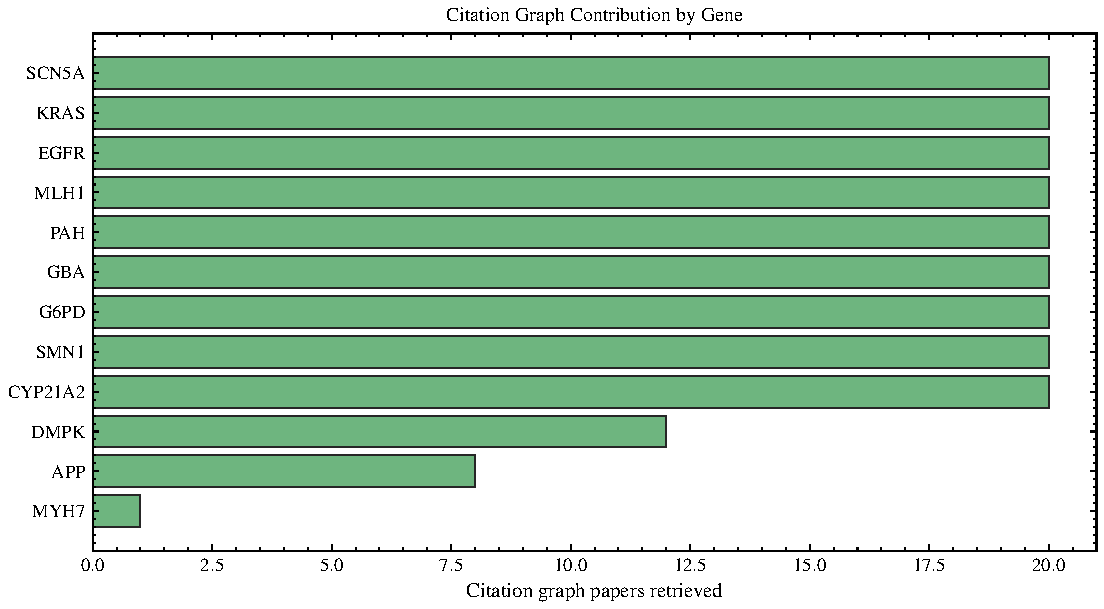
\includegraphics[width=\columnwidth]{fig4_citation_graph.pdf}
  \caption{Citation graph traversal per gene (nested pipeline): papers
  retrieved vs.\ reference-set relevant. The dotted line marks the
  traversal budget (20 papers per variant); relevant contributions
  concentrate in EGFR (5), DMPK (5), and PAH (1).}
  \label{fig:citation}
\end{figure}

\subsection{Reproducibility and Released Artifacts}
\label{sec:repro}

We release, alongside the MIT-licensed system code: the reference set
(30 variants, 540 annotations with language and evidence-type fields); the
raw per-method ranked candidate lists exactly as collected (2026-08-12,
12:09--13:47 local, single session); the collection log (78 Semantic
Scholar HTTP-429 events, 120 J-STAGE parse failures, 60 translation
calls); the translation system prompt (temperature 0.2, six target
languages) whose SHA-256 fingerprint is embedded in the released run
manifest; and a deterministic analysis script
(\texttt{make\_paper\_data.py}) that regenerates every table, figure, and
statistic in this paper from the raw lists, including the nested-M4
construction, the Holm-corrected test family, and bootstrap CIs (10{,}000
resamples, fixed seed 42). The benchmark runner records a machine-readable
manifest (configuration echo, model identifiers, per-variant timings,
budgets) for future collection runs; the LLM endpoint used for the
2026-08-12 translation run was configured via environment and its
identifier was not captured by the original log --- a reproducibility gap
we document rather than obscure, and which the manifest now closes for
subsequent runs. All retrieval-dependent results reflect live-API state in
the stated collection window.

\section{Discussion}
\label{sec:discussion}

\textbf{Limitations.} In order of severity: (i) \emph{Reference-set
construct validity is the binding constraint on every conclusion}: the
annotations are heuristic, expert-unverified, and drawn from a candidate
pool whose channels overlap the evaluated system
(Section~\ref{sec:goldstd}); metrics are relative coverage of that pool,
and genuinely clinical claims (e.g., PS3/PVS1 evidence retrieval quality)
are out of reach of this evaluation. (ii) Candidate budgets in the
recorded runs were 14.2--26 per variant (client caps and rate limits),
below the $K{=}50$ originally advertised; we therefore report fixed-$K$
metrics only within budget and label set-level metrics as such, and the
corrected runner defaults to uniform 50-candidate budgets. (iii) All
online results are single runs; the measured run-to-run jitter
(Section~\ref{sec:variance}) is of the same order as the component
deltas, so per-component conclusions are preliminary. (iv) The relevance
gate, OA download layer, health-aware scheduling, and deduplication
accuracy are engineering features without dedicated experiments here
(gating accuracy/cost, download success and license correctness,
fault-injection behavior, and dedup precision/recall are each unmeasured).
(v) Language metadata is missing for 228 reference papers, and only
German/French carry non-English annotations. (vi) The external baselines
of Section~\ref{sec:external} were collected one day after the main runs;
cross-snapshot comparisons carry that caveat.

\textbf{Future work.} Expert re-annotation is the priority: dual
independent annotation with clinical-genetics expertise on a stratified
sample of pooled candidates (including candidates from systems that do
not share our providers), adjudication, and reported inter-annotator
agreement (Cohen's $\kappa$), distinguishing ``about the gene/disease''
from ``usable as variant-level evidence''. Protocol-side: a full re-run
under the corrected uniform-budget nested protocol; per-language
translation fidelity evaluation (gene-symbol and HGVS retention rates,
now measurable since the runner persists translated queries); dedicated
experiments for the gate (precision/recall/cost on human labels),
download layer (OA resolution success, license correctness, valid-PDF
rate), health scheduler (fault injection), and deduplication
(precision/recall on retained raw streams); and embedding-based semantic
retrieval as an additional recall channel.

\section{Conclusion}
\label{sec:conclusion}

We presented lit-acquisition, an open-source multi-source multilingual
biomedical literature acquisition system, together with an exploratory,
heuristically annotated reference set and a corrected evaluation protocol
(strictly nested ablation, budget-honest fixed-$K$ metrics, Holm-corrected
paired statistics, quantified run-to-run API variance, and transparent
fusion baselines). On this reference set the end-to-end pipeline roughly
doubles PubMed-only set recall (0.171 $\rightarrow$ 0.345, Holm-adjusted
$p{=}0.004$); individual component contributions are positive but not
individually significant at $n{=}30$, translation recovers 21 of 24
annotated German/French papers in a controlled contrast, and citation
traversal adds a small set of otherwise-unretrieved papers on 3 variants
at a significant list-level precision cost. We position this work as
infrastructure --- code, unified provider interfaces, raw run data, and a
deterministic analysis pipeline --- for the community to build clinically
validated evaluations on, not as evidence of clinical retrieval quality;
the reference set requires expert re-annotation before any such claim.

\bibliographystyle{ACM-Reference-Format}
\begin{thebibliography}{99}

\bibitem{richards2015standards}
S.~Richards et al.
\newblock Standards and guidelines for the interpretation of sequence
variants: a joint consensus recommendation of the ACMG and the AMP.
\newblock \emph{Genetics in Medicine}, 17(5):405--424, 2015.

\bibitem{pubmed}
E.~Sayers et al.
\newblock Database resources of the National Center for Biotechnology
Information.
\newblock \emph{Nucleic Acids Research}, 50(D1):D20--D26, 2022.

\bibitem{europepmc}
The Europe PMC Consortium.
\newblock Europe PMC: a full-text literature database for the life sciences
and platform for innovation.
\newblock \emph{Nucleic Acids Research}, 43(D1):D1042--D1048, 2015.

\bibitem{kinney2023semantic}
R.~Kinney et al.
\newblock The Semantic Scholar Open Data Platform.
\newblock \emph{arXiv preprint arXiv:2301.10140}, 2023.

\bibitem{mastermind}
Genomenon.
\newblock Mastermind Genomic Search Engine.
\newblock \url{https://www.genomenon.com/mastermind/}.

\bibitem{covidence}
Veritas Health Innovation.
\newblock Covidence systematic review software.
\newblock \url{https://www.covidence.org/}.

\bibitem{ouzzani2016rayyan}
M.~Ouzzani, H.~Hammady, Z.~Fedorowicz, and A.~Elmagarmid.
\newblock Rayyan---a web and mobile app for systematic reviews.
\newblock \emph{Systematic Reviews}, 5(1):210, 2016.

\bibitem{selberg1997metacrawler}
E.~Selberg and O.~Etzioni.
\newblock The MetaCrawler architecture for resource aggregation on the
World Wide Web.
\newblock \emph{IEEE Expert}, 12(3):11--14, 1997.

\bibitem{priem2022openalex}
J.~Priem, H.~Piwowar, and R.~Orr.
\newblock OpenAlex: a fully-open index of scholarly works, authors, venues,
institutions, and concepts.
\newblock \emph{arXiv preprint arXiv:2205.01833}, 2022.

\bibitem{kessler1963bibliographic}
M.~M. Kessler.
\newblock Bibliographic coupling between scientific papers.
\newblock \emph{American Documentation}, 14(1):10--25, 1963.

\bibitem{small1973co}
H.~Small.
\newblock Co-citation in the scientific literature: a new measure of the
relationship between two documents.
\newblock \emph{Journal of the American Society for Information Science},
24(4):265--269, 1973.

\bibitem{page1999pagerank}
L.~Page, S.~Brin, R.~Motwani, and T.~Winograd.
\newblock The PageRank citation ranking: bringing order to the web.
\newblock Technical report, Stanford InfoLab, 1999.

\bibitem{swanson1986fish}
D.~R. Swanson.
\newblock Fish oil, Raynaud's syndrome, and undiscovered public knowledge.
\newblock \emph{Perspectives in Biology and Medicine}, 30(1):7--18, 1986.

\bibitem{kishida2005technical}
K.~Kishida.
\newblock Technical issues of cross-language information retrieval: a review.
\newblock \emph{Information Processing \& Management}, 41(3):433--455, 2005.

\bibitem{brown2020language}
T.~Brown et al.
\newblock Language models are few-shot learners.
\newblock In \emph{Advances in Neural Information Processing Systems 33},
2020.

\bibitem{kojima2022large}
T.~Kojima, S.~Gu, M.~Reid, Y.~Matsuo, and Y.~Iwasawa.
\newblock Large language models are zero-shot reasoners.
\newblock In \emph{Advances in Neural Information Processing Systems 35},
22199--22213, 2022.

\bibitem{jarvelin2002cumulated}
K.~J\"arvelin and J.~Kek\"al\"ainen.
\newblock Cumulated gain-based evaluation of IR techniques.
\newblock \emph{ACM Transactions on Information Systems}, 20(4):422--446,
2002.

\bibitem{wilcoxon1945individual}
F.~Wilcoxon.
\newblock Individual comparisons by ranking methods.
\newblock \emph{Biometrics Bulletin}, 1(6):80--83, 1945.

\bibitem{holm1979simple}
S.~Holm.
\newblock A simple sequentially rejective multiple test procedure.
\newblock \emph{Scandinavian Journal of Statistics}, 6(2):65--70, 1979.

\bibitem{cormack2009reciprocal}
G.~V. Cormack, C.~L.~A. Clarke, and S.~B\"uttcher.
\newblock Reciprocal rank fusion outperforms Condorcet and individual
rank learning methods.
\newblock In \emph{Proceedings of SIGIR}, 758--759, 2009.

\bibitem{unpaywall2018}
H.~Piwowar, J.~Priem, V.~Larivi\`ere, J.~P. Alperin, L.~Matthias,
B.~Norlander, A.~Farley, J.~West, and P.~Haustein.
\newblock The state of OA: a large-scale analysis of the prevalence and
impact of Open Access articles.
\newblock \emph{PeerJ}, 6:e4375, 2018.

\bibitem{ginsparg1994arxiv}
P.~Ginsparg.
\newblock First steps towards electronic research communication.
\newblock \emph{Computers in Physics}, 8(4):390--396, 1994.

\bibitem{doaj}
Directory of Open Access Journals.
\newblock \url{https://doaj.org/}.

\bibitem{cinii}
National Institute of Informatics.
\newblock CiNii Research.
\newblock \url{https://cir.nii.ac.jp/}.

\bibitem{jstage}
Japan Science and Technology Agency.
\newblock J-STAGE.
\newblock \url{https://www.jstage.jst.go.jp/}.

\bibitem{scielo}
SciELO.
\newblock Scientific Electronic Library Online.
\newblock \url{https://scielo.org/}.

\bibitem{base}
Bielefeld University Library.
\newblock BASE -- Bielefeld Academic Search Engine.
\newblock \url{https://www.base-search.net/}.

\bibitem{core}
CORE.
\newblock Aggregate of open access research papers.
\newblock \url{https://core.ac.uk/}.

\bibitem{openaire}
OpenAIRE.
\newblock \url{https://www.openaire.eu/}.

\bibitem{zenodo}
CERN.
\newblock Zenodo -- Research. Shared.
\newblock \url{https://zenodo.org/}.

\bibitem{zarin2016clinicaltrials}
D.~A. Zarin, T.~Tse, R.~J. Williams, and S.~Carr.
\newblock Trial reporting in ClinicalTrials.gov -- the Final Rule.
\newblock \emph{New England Journal of Medicine}, 375(20):1998--2004, 2016.

\end{thebibliography}

\end{document}
